% \documentclass[10pt, oneside, english]{article}   	
\documentclass[10pt, oneside]{article}
\usepackage{geometry}                		
\geometry{a4paper}                   		
% \usepackage[english, es-noindentfirst]{babel}
% \selectlanguage{english}
\usepackage[utf8]{inputenc}               		
\usepackage{graphicx}			
\usepackage{amssymb}
\usepackage{authblk}
\usepackage{multicol}
\usepackage{rotating}


\title{Word embeddings for predicting political affiliation based on Twitter data}
\author[]{Ibrahim Abdelaziz}
\author[]{Oliver Berg}
\author[]{Angjela Davitkova}
\author[]{Venkatesh Iyer}
\author[]{Shriram Selvakumar}
\author[]{Kumar Shridhar}
\author[]{Saurabh Varshneya}
\affil[1]{Technische Universität Kaiserslautern}




\begin{document}
\maketitle
\begin{multicols}{2}


\section{Introduction}

The modern world of social media knows a plethora of means to communicate ones personal opinion and political alignment. With the platform \textit{Twitter}, figures of political interest are expressing their standpoints in small-sized 144 -character texts (recently updated to 280 characters), which contain a comprised message specific to the general public. This yields great potential for automated analysis of party affiliations to classify political persons of interest within the overall political spectrum \cite{Biessmann2017}.

Hence, we propose a structured approach of building a deep learning based classification model that utilizes state-of-the-art \textbf{word embeddings} \cite{Pelevinala2016} to perform \textbf{qualitative analysis} on constructed \textbf{social media data set}. Our approach will be helpful in analyzing possible early intuitions and dedicated insights within German political spectrum.
This is to be seen in context of latest \textbf{advances in research}.

\section{Data Sets and Feature Extraction} 

Political motives were shown to be consistently predictable with an accuracy better than chance \cite{Biessmann2017}.
According to the presented task description of analyzing political affiliation based on Twitter-data, \textbf{tweets} made by political figures on the platform Twitter were used for the findings.
Additionally, categorized data set taken from \textit{www.wahl.de/politiker} may be leveraged as a prearrangement of the initial raw Twitter-data.

For the purpose of this specific research, the main portion of data would be the Twitter data. In order to include all of the relevant politicians from the parties, their corresponding Twitter accounts will be collected (Twitter, wahl.de), where the data is offered as open source data.
For each of the Twitter accounts of the politicians, a corresponding party is kept, for which the politician is working. Having these accounts, the same number of tweets will be crawled for each of the parties. 80 percent of the collected data would be used from training the classifier and 20 percent of it would be used for testing.
Additionally, for more testing purposes, the previously mentioned data sources, that includes parliament discussion data and party manifesto data, can be used. 

In order to train models on text, the data needs to be converted into numerical values, more specifically vectors, under specific similarity metrics. One way this can be achieved is to create a word embedding for each of the words from the tweets using \textit{Word2Vec}. While constructing word embeddings, appropriate dimensionality reduction can be applied.


\section{Recent Developments}

Existing papers \cite{Misra20XX} then tackle the classification problem using various techniques, such as SVM, SVD or LSM. Mainly these approaches consider solely the political affiliation in America, where the orientation is rather simpler, since there are only two sides and the users are mainly biased towards one side. 
Other sources tend to focus on comparison of different classifiers when trying to tackle this problem, and thus not proposing a complete well-developed approach \cite{Bhanda2009}.
Overall, sentiment classification is mostly covered using recurrent- or convolutional neural networks \cite{Kim2014}.

In connection to the given focus of working on Twitter data, \cite{Cohen20XX} introduces objections to some of the preexisting approaches. With standard classifiers for inferring political orientation having greatly lower accuracy from the accuracy that they report, it is stated that the classifiers cannot be used for classifying users outside the training data. Thus the contradictory arguments hold true.

\section{Proposed Methodology}

Using a recurrent neural network architecture (LSTM) seems a good solution for our specific task. Since the twitter dataset is very complex (giving it's small length and more information), a recurrent neural network alone will be unable to learn all the features. So, a convolutional neural network at the start can be used to learn character wise information before the words are fed to a recurrent neural network that learns the context within data.

The proposed solution will leverage neural networks, where we compare different approaches of both convolutional- and recurrent networks architectures.


\section{Analysis of Results}

For the results analysis, various metrics can be used with primary ones being Pearson Correlation Coefficient, F1-Score and Cosine Similarities. Further more, clustering of data can be done to find the outliers within the embedding space. Visualization techniques like T-SNE and PCA can be used to visualize the results. 

\bibliography{lit}
\bibliographystyle{plain}

\end{multicols}

\newpage
\section{Appendix - Work packages and distribution}

We plan to distribute the workload into the work packages, for each work package we assign a group of people, and an initial estimated deadline.

\begin{flushleft}
\textbf{Building dataset}

Beside the Tweets of German politicians that we will get using the Twitter API, we also plan to collect data from other sources such as parliament discussion data and party manifesto data.
\end{flushleft}

\begin{flushleft}
\textbf{Training word vector model}

After building our dataset we will convert the data text into numerically creating word embedding of the words in the text using Word2Vec or derived approaches.
\end{flushleft}

\begin{flushleft}
\textbf{Developing classification model}

As previously mentioned in the Proposed Methodology we will implement a neural network as our classifier, and train it with our data set.
\end{flushleft}

\begin{flushleft}
\textbf{Training / Testing}

After having quantified model accuracy with a dedicated validation split, this separate training- and testing-stage ensures that the obtained results match initial expectations or reject estimates in an understandable fashion. We thereby ensure that the obtained results obey logic and real-world measures.
\end{flushleft}

\begin{flushleft}
\textbf{Quantitative Analysis}

To conclude the findings from real-word social media data analysis, we infer statistical and sociological meaning to the modeled results and put them in context to the initially motivated research question of political affiliation and political classification.
\end{flushleft}

\begin{sidewaysfigure}
  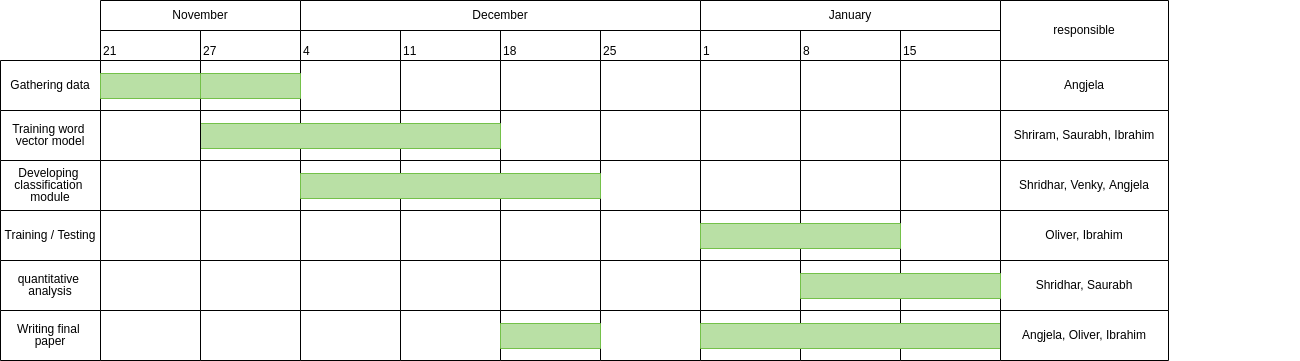
\includegraphics[width=\textwidth]{gantt.png}
  \caption{Gantt-Chart displaying workload distribution per team-member}
\end{sidewaysfigure}

\end{document} 
